\documentclass{article}

\usepackage[final, nonatbib]{nips_2017}

\usepackage[utf8]{inputenc} % allow utf-8 input
\usepackage[T1]{fontenc}    % use 8-bit T1 fonts
\usepackage{hyperref}       % hyperlinks
\usepackage{url}            % simple URL typesetting
\usepackage{booktabs}       % professional-quality tables
\usepackage{amsfonts}       % blackboard math symbols
\usepackage{nicefrac}       % compact symbols for 1/2, etc.
\usepackage{microtype}      % microtypography
\usepackage{pgfplots}       % bar graphs

\title{Text Classification Using a Single Layer Convolutional Neural Network}

\author{
  Remington Thurber \\
  Department of Mathematics and Computer Science \\
  South Dakota School of Mines \& Technology \\
  Rapid City, SD 57701 \\
  \texttt{remington@remolten.com} \\
}

\begin{document}

\maketitle

\begin{abstract}
This paper presents a deep learning network for text classification of the 20 newsgroups dataset, with the goal of achieving
90\% testing accuracy. To accomplish this, it uses a convolutional
neural network (CNN). The CNN utilizes a single layer of convolution, max pooling, dropout, and other optimization techniques.
The network achieves 54\% accuracy on the test data and 99\% accuracy on the training data, when tested over 100 epochs.
Thus, it fails to reach the expected testing accuracy.
This paper concludes by suggesting the usage of a deeper CNN and pre-trained word embeddings in order to improve classification accuracy.
\end{abstract}

\section{Introduction}
Natural language processing (NLP) is an important problem that machine learning is well suited to solve. The uses for NLP are many:
text classification, sentiment analysis, determining the relations between words, and even generating responses to questions.
Most deep learning approaches today use either CNN's, or recurrent neural networks (RNN's) to solve the this problem.

CNN's perform well on text classification problems because they function as feature extractors \cite{zhang}. So, when
applied to text, CNN's can be used to find specific words or a sequence of words. Another advantage of CNN's is that they can extract features
from any location in the input data \cite{goldberg}. Essentially, when the network learns an important word or sequence of words,
the CNN is able to always identify these features, no matter where they appear in a paragraph or document.

In this paper, I present a single layer CNN to solve the problem of text classification on the 20 newsgroups dataset. This single layer CNN
uses word embeddings to represent its inputs. Word embeddings are essentially multi-dimensional representations of
words, where similar words have a similar representation. There are pre-trained word embeddings available for use in machine learning,
including GloVe and word2vec. These generally provide superior performance, because they are pre-trained to understand the relations
between words in general, not just when applied to a single problem. However, it also can be advantageous to simply learn these word
embeddings, because more useful relations can be found when applied directly to a specific problem; in this case, text classification.
Single layer CNN's generally perform fairly well for most text classification tasks, especially when used with pre-trained word
embeddings \cite{kim} \cite{goldberg}. My network does not use pre-trained word embeddings.

However, there are some downsides to using CNN's. CNN's are especially sensitive to hyperparameters, when compared to other types of neural
networks \cite{zhangwallace}. As such, they require much work from the programmer to tune the network
to achieve optimal performance. For the new machine learning programmer, it can be difficult to know exactly what to select, because the
entire network, including the hyperparameters, seems like magic.

\subsection{The Dataset}
Text classification will be done on the 20 newsgroups dataset. The data is a collection of forum posts, that each belong to a
different sub-forum. Some of the categories include 'rec.autos', 'sci.crypt', 'alt.atheism', and 'soc.religion.christian'. In total, there
are 20 categories, with some of them being very similar. Thus, this is considered to be a fairly difficult text classification problem for
deep learning.

\section{Methods}
In this section, I explain how my CNN was constructed, including data preprocessing and the network architecture itself.

\subsection{Deep Learning Framework}
TensorFlow v1.7.0 was used to create the network and the Numpy package was used for data manipulation. Finally, the Sklearn package was used
to obtain the 20 newsgroups dataset.

\subsection{Preprocessing Data}
The dataset was read into the program as a sequence of strings, and the expected categories. Then, the data was processed to support input
and output to and from the network.

First, the input data was processed to support a bag-of-words model. To do this, each word in the dataset was assigned a unique integer
identifier. Then, the network's input was a sequence of those identifiers, corresponding to their respective words in each document. So,
the amount of inputs was the size of the largest document. This was found to be very expensive for training time. Instead, the
amount of inputs was capped to 500, and any documents with more than 500 words were truncated. Any shorter documents used 0, the pad word,
as their extra inputs. Finally, the input data was further cleaned by only keeping alphanumeric characters.

The output data was processed to support one hot encoding. The expected output of each data sample is a probability distribution of size
20 (the number of classes), with 1 in the index of the expected category, and 0 elsewhere.

A train to test data ratio of 80:20 was chosen, which was found to be optimal for testing accuracy. Also, the data was shuffled each epoch
in order to improve the robustness of the network.

\subsection{Network Architecture}
A CNN was utilized. It consisted of an input + embedding layer, a convolution layer, a max pooling layer, and a fully connected output layer.

\subsubsection{Input + Embedding Layer}
The data was fed into the network using a bag-of-words model. Then, in this layer, the unique integer identifiers were
converted to word embeddings of size 75. These embeddings are randomly initialized using a uniform distribution, and were learned by the
network. Finally, the dimensionality of the data was increased to 4 dimensions, in preparation for spatial convolution.

\subsubsection{Convolution Layer}
The convolution layer used a stride of 1 with 3 filter sizes: 1, 2, and 3. Filters were initialized using a truncated normal initializer for
the weights and a random normal initializer for the biases. Then, convolution was performed with a total of 150 filters
per filter size. Finally, the data was passed through a Leaky ReLU activation function. Other activation functions were tried,
including ReLU, tanh, and sigmoid. Generally, they generated inferior results or significantly increased the training time, when compared
to Leaky ReLU. Varying the alpha value for Leaky ReLU did not change the accuracy much, so the default of 0.2 was used.

\subsubsection{Max Pooling Layer}
After convolution, max pooling was performed over each document, with a stride of 1. This generated 450 outputs for each input document.
Before passing to the next layer, dropout was performed, with a dropout rate of 0.5.

\subsubsection{Fully Connected Output Layer}
The final output layer was fully connected. It reduced the 450 outputs from the max pooling to a probability distribution of 20 classes.
I experimented with using multiple fully connected layers, but it slowed the training time and did not increase the accuracy of the network
in any meaningful amount.

\subsection{Network Optimization}

\subsubsection{Mini-Batches}
Throughout the training process, data was split into random mini-batches in order to enable parallelism and increase the overall perfomance of
the network. A batch size of 50 was selected, in order to keep the GPU memory requirements reasonable. Experimentation was done with other batch
sizes, but it caused little difference in accuracy.

\subsubsection{Loss Function}
The outputs were passed through a softmax function, and then used to calculate the cross entropy. This loss function is appropriate for the
task because the outputs are a probability distribution.

\subsubsection{Optimizer}
The Adam optimization algorithm was found to be the best for the task, because it trained the fastest. A basic gradient descent optimizer and the Adagrad
algorithm were also tried, but produced inferior results and increased the training time.

\subsubsection{Weight Regularization}
L2 loss was used as a method of weight regularization. Through experimentation, a value of 0.0001 was selected for the L2 lambda value.
No other regularization algorithms were tried. It provided a minor benefit to accuracy.

\section{Results}
The network achieved approximately 95\% accuracy on the training data and 50\% accuracy on the testing data, when trained over 10 epochs. When trained
for 100 epochs or more, it would converge to around 99\% accuracy on the training data and 54\% accuracy on the testing data.

I experimented with changing various hyperparameters to optimize accuracy—including filter sizes and word embedding sizes.

\begin{table}[b]
  \caption{Varying Filter Sizes}
  \label{tab:filter_sizes}
  \centering
  \begin{tabular}{ccc}
    \toprule
    Filter Sizes & Test Accuracy (10 epochs) & Train Accuracy (10 epochs) \\
    \midrule
    1, 2, 3 & 0.5138888909584947 & 0.925363634662194 \\
    1, 2, 4 & 0.5169444448418088 & 0.936090906099839 \\
    2, 3, 4 & 0.4855555531879266 & 0.910363632440567 \\
    2, 3, 5 & 0.4805555554727713 & 0.910999996824698 \\
    2, 3, 7 & 0.4927777755591604 & 0.915909086574207 \\
    3, 4, 5 & 0.4038888886570930 & 0.820636357773434 \\
    4, 5, 6 & 0.2844444442954328 & 0.682272729954936 \\
    \bottomrule
  \end{tabular}
\end{table}

Table~\ref{tab:filter_sizes} shows various filter sizes that were tried, and their respective final accuracies when trained over 10 epochs.
The default embedding size of 75 was used.
The filter size of 2 appears to have caused the greatest difference in accuracy. Further, choosing the smaller filter sizes generally
produced the best results.

\begin{table}
  \caption{Varying Embedding Sizes}
  \label{tab:embedding_sizes}
  \centering
  \begin{tabular}{ccc}
    \toprule
    Embedding Sizes & Test Accuracy (10 epochs) & Train Accuracy (10 epochs) \\
    \midrule
    50 & 0.509722221228811 & 0.927636359225619 \\
    75 & 0.513888890958494 & 0.925363634662194 \\
    100 & 0.522222220483753 & 0.940090905265374 \\
    150 & 0.519722222867939 & 0.939181814410469 \\
    200 & 0.519722221626175 & 0.932272725213657 \\
    300 & 0.531944442954328 & 0.948272725939750 \\
    400 & 0.540277776204877 & 0.946454542333429 \\
    \bottomrule
  \end{tabular}
\end{table}

Table~\ref{tab:embedding_sizes} shows various embedding sizes that were tried. The default filter sizes of 1, 2, and 3 were used.
As the results show, it seems that embeddings between sizes 50 and 200 had similar accuracy. Larger embeddings of size 300 or 400
provided the best accuracy at the cost of training speed.

\begin{figure}[h]
    \centering
    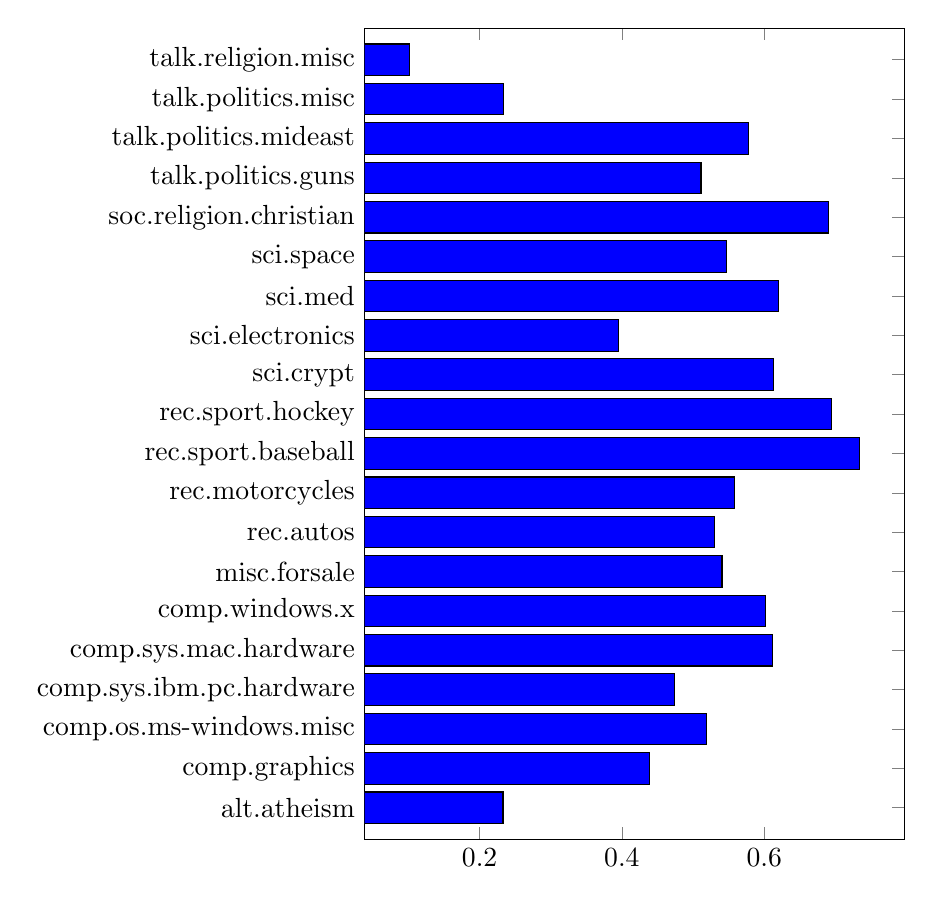
\begin{tikzpicture}
        \begin{axis}[
            symbolic y coords={alt.atheism, comp.graphics, comp.os.ms-windows.misc, comp.sys.ibm.pc.hardware, comp.sys.mac.hardware,
                               comp.windows.x, misc.forsale, rec.autos, rec.motorcycles, rec.sport.baseball, rec.sport.hockey, sci.crypt,
                               sci.electronics, sci.med, sci.space, soc.religion.christian, talk.politics.guns, talk.politics.mideast,
                               talk.politics.misc, talk.religion.misc},
            ytick=data,
            bar width=4mm,
            y=5mm,
            enlarge y limits={abs=4mm}
            ]
            \addplot[xbar,fill=blue] coordinates {
                (0.23287672,alt.atheism)
                (0.43850267,comp.graphics)
                (0.5185185,comp.os.ms-windows.misc)
                (0.47395834,comp.sys.ibm.pc.hardware)
                (0.6121212,comp.sys.mac.hardware)
                (0.60215056,comp.windows.x)
                (0.54066986,misc.forsale)
                (0.5297297,rec.autos)
                (0.55837566,rec.motorcycles)
                (0.7336956,rec.sport.baseball)
                (0.69518715,rec.sport.hockey)
                (0.61256546,sci.crypt)
                (0.39473686,sci.electronics)
                (0.62051284,sci.med)
                (0.5464481,sci.space)
                (0.69072163,soc.religion.christian)
                (0.51111114,talk.politics.guns)
                (0.578125,talk.politics.mideast)
                (0.23417722,talk.politics.misc)
                (0.1015625,talk.religion.misc)
            };
        \end{axis}
    \end{tikzpicture}
    \caption{Individual Classes Accuracy}
    \label{fig:classes_accuracy}
\end{figure}

Figure~\ref{fig:classes_accuracy} shows how the network performed on each of the categories in the dataset. The best performance occurred on
rec.sport.baseball, rec.sport.hockey, and soc.religion.christian. Conversely, the network performed the worst when classifying
talk.religion.misc, alt.atheism, and talk.politics.misc.

\section{Discussion}
\subsection{Analysis of Results}
The 54\% testing accuracy achieved failed to reach the goal of 90\%. There are a few reasons why this could have occurred.
Firstly, it's possible that the network is overfitting. However, from my testing, I do not think that is the case. Most likely, the low
accuracy was a result of the network architecture being too simple.

To combat this issue, I experimented with deeper architectures—multiple layers of convolution and max pooling—but I failed to get the
implementation functioning above 5\% accuracy. In addition, increasing the depth also exponentially increased the training time, so I was not
able to easily test whether or not the network was working properly. Overall, I do think that a deep CNN, possibly paired with additional
fully connected layers, would be the best solution to the problem, and experimental findings by Zhang et al. \cite{zhang} seem to confirm this.

It was also found that the filter sizes of 1, 2, and 3 were the most optimal. Further, it seems that the filter sizes of 1 and 2 were the most
important, because any tests performed without them had significantly lower accuracy. There are several interpretations for why this could
have occurred. One possible reason is that some of the documents have single or double words that are a sure indicator of the class. So, when the
small filter sizes are missing, combining these single or double words into larger sequences distorts their meanings. Finally, when only filter sizes
of 3 or higher were used, there was a significant reduction in performance. This probably indicates that longer sequences of words are not as
important as shorter sequences, or single words.

While experimenting with different embedding sizes, it seemed that embedding sizes in the range of 50 to 200 performed similarly. I ended up
selecting a size of 75 because it balanced fast training times with good accuracy. It seemed like
larger word embeddings, of sizes 300 or 400, produced better results, but there was a high cost to the training time. I hypothesize that
increasing the size of the word embeddings would continually increase performance, but with diminishing returns and a large expense to the
training time.

Finally, there was a large variance in classification accuracy among the different categories. I hypothesize that most of the best performing
categories, like rec.sport.hockey, contain distinct words or sequences of words that easily differentiate those documents from the other
categories. This makes sense, especially considering that the sports categories, which have lots of distinct jargon, had great performance.
On the other hand, some of the poorly performing categories were the miscellaneous categories: talk.religion.misc and talk.politics.misc. I
hypothesize that these categories were difficult to categorize because they contain a wide array of information. So, there is not a word or
sequence of words that occur frequently within these categories, which causes the network to have trouble categorizing them.

\subsection{Future Work}
Unfortunately, due to time constraints, I was unable to utilize pre-trained word embeddings. My initial goal was to use GloVe as
the initial values for the embeddings, and then continue to optimize them with learning. In addition, I would like to get
multi-layer convolution working; which, when combined with pre-trained word embeddings, would probably increase the testing classification accuracy
to 90\% or above. Finally, I would also like to experiment more with additional fully connected layers. Though my initial experimentation
suggested that only 1 fully connected layer was needed, I still think there is potential for an increase in accuracy with more of these layers.

\newpage

\begin{thebibliography}{9}

\bibitem{zhang}
Xiang Zhang, Junbo Zhao, and Yann LeCun.  Character-level Convolutional Networks for Text Classification.
https://arxiv.org/abs/1509.01626

\bibitem{kim}
Yoon Kim.  Convolutional Neural Networks for Sentence Classification.
https://arxiv.org/abs/1408.5882

\bibitem{goldberg}
Yoav Goldberg. A Primer on Neural Network Models for Natural Language Processing.
https://arxiv.org/abs/1510.00726

\bibitem{zhangwallace}
Ye Zhang and Byron Wallace. A Sensitivity Analysis of (and Practitioners' Guide to) Convolutional Neural Networks for Sentence Classification.
https://arxiv.org/abs/1510.03820

\end{thebibliography}

\end{document}
